\chapter{Numerical results}
\vspace{-8mm}
In the previous chapter, we discuss the implementation details
and how we implement and apply LBM to various settings.
In this chapter, we show the visualizations and numerical results
obtained from the series experiments.

\section{Validation experiments}
In the physics simulation, it is always important
to validate whether the implementation is correct.
Therefore, we first show how to validate the implementation
using several examples.

\subsection{Shear wave decay}
The shear wave decay represents the time evolution of a
velocity perturbation in the flow.
Since the viscosity decays the velocity of the flow,
the velocity converges to zero in the end.
When we set the following sinusoidal perturbation in the velocity
as the initial condition:
\begin{equation}
  \begin{aligned}
    \uv(\xv, t = 0) =
    \begin{bmatrix}
      u_x(y, t = 0) \\
      0 \\
    \end{bmatrix}
    =  
    \begin{bmatrix}
      \epsilon \sin \frac{2\pi y}{Y} \\
        0 \\
      \end{bmatrix}
  \end{aligned}
  \label{shear-vel-init}
\end{equation}
Then the analytical solution for the time evolution of 
the velocity is calculated as follows~\cite{fei2018three}:
\begin{equation}
  \begin{aligned}
    u_x(y, t) &= 
    \epsilon \exp\biggl(
      -\nu \biggl(
        \frac{2\pi}{Y}
      \biggr)^2 t\biggr) \sin \frac{2\pi y}{Y}
  \end{aligned}
  \label{sinusoidal-vel-analytical-solution}
\end{equation}
Note that this result is obtained using Navier-Stokes equations for incompressible fluid
and the assumptions that the pressure term $\nabla p$ and
the convection term $(\uv \cdot \nabla) \uv$ are negligible 
compared to the viscosity term $\nu \nabla^2 \uv$.
In Figure~\ref{fig:sinusoidal-velocity}, we show the plot of both
simulated results and the analytical solutions of sinusoidal velocity.
Note that the initial condition follows Eq~(\ref{shear-vel-init}). 
As seen in the figure, the simulated results and the analytical solutions
{\bf perfectly fit} and thus we could validate our implementation of
rigid wall and moments updates.
Figure~\ref{fig:sinusoidal-density} shows the density distribution
over time.
This simulation uses the sinusoidal density in $x$-direction:
\begin{equation}
\begin{aligned}
  \rho(\xv, 0) = \rho_0 + \epsilon \sin \frac{2 \pi x}{X}
\end{aligned}
\end{equation}

\begin{figure}[H]
  \begin{center}
    \subfloat[$t = 0$]{
      \includegraphics[width=0.23\textwidth]{../log/sinusoidal_velocity/fig/vel000000.pdf}
    }
    \subfloat[$t = 200$]{
      \includegraphics[width=0.23\textwidth]{../log/sinusoidal_velocity/fig/vel000200.pdf}
    }
    \subfloat[$t = 400$]{
      \includegraphics[width=0.23\textwidth]{../log/sinusoidal_velocity/fig/vel000400.pdf}
    }
    \subfloat[$t = 600$]{
      \includegraphics[width=0.23\textwidth]{../log/sinusoidal_velocity/fig/vel000600.pdf}
    }\\
    \vspace{-3mm}
    \subfloat[$t = 800$]{
      \includegraphics[width=0.23\textwidth]{../log/sinusoidal_velocity/fig/vel000800.pdf}
    }
    \subfloat[$t = 1000$]{
      \includegraphics[width=0.23\textwidth]{../log/sinusoidal_velocity/fig/vel001000.pdf}
    }
    \subfloat[$t = 1200$]{
      \includegraphics[width=0.23\textwidth]{../log/sinusoidal_velocity/fig/vel001200.pdf}
    }
    \subfloat[$t = 1400$]{
      \includegraphics[width=0.23\textwidth]{../log/sinusoidal_velocity/fig/vel001400.pdf}
    }\\
    \vspace{-3mm}
    \subfloat[$t = 1600$]{
      \includegraphics[width=0.23\textwidth]{../log/sinusoidal_velocity/fig/vel001600.pdf}
    }
    \subfloat[$t = 1800$]{
      \includegraphics[width=0.23\textwidth]{../log/sinusoidal_velocity/fig/vel001800.pdf}
    }
    \subfloat[$t = 2000$]{
      \includegraphics[width=0.23\textwidth]{../log/sinusoidal_velocity/fig/vel002000.pdf}
    }
    \subfloat[$t = 2200$]{
      \includegraphics[width=0.23\textwidth]{../log/sinusoidal_velocity/fig/vel002200.pdf}
    }\\
    \caption{The velocity evolution for the sinusoidal velocity at
      the $x = 25$ in the lattice grid size of $(50, 50)$.
      The $x$-axis shows the location in the $y$ direction
      and the $y$-axis shows the magnitude of velocity at 
      the corresponding location.
      The coefficients $\epsilon$ and the initial density $\rho_0$ are 
      set to $0.01$ and $1.0$ respectively.
      The relaxation term $\omega$ are set to $1.0$.
      \label{fig:sinusoidal-velocity}}
  \end{center}
\end{figure}

Additionally, we obtain the following equation regarding the viscosity by
transforming Eq~(\ref{sinusoidal-vel-analytical-solution}):
\begin{equation}
  \begin{aligned}
    u_x(y, t) &= \epsilon
    \Biggl(
    -\nu
    \biggl(
      \frac{2\pi}{Y}
      \biggr)^2 t
    \Biggr) 
    \sin  \frac{2\pi y}{Y} \exp
      \Longleftrightarrow 
    \frac{u_x(y, t)}{
      \epsilon
      \sin  \frac{2\pi y}{Y}
    }  =  \exp
    \Biggl(
    -\nu
    \biggl(
      \frac{2\pi}{Y}
      \biggr)^2 t
    \Biggr) \\
    -\nu
    \biggl(
      \frac{2\pi}{Y}
      \biggr)^2 t
      &= 
    \log \frac{u_x(y, t)}{
      \epsilon
      \sin  \frac{2\pi y}{Y}
    }~(\text{Take log of both sides}) \\
    \nu
      &=
      - \frac{1}{t}
      \biggl(
        \frac{Y}{2\pi}
        \biggr)^2 
    \log \frac{u_x(y, t)}{
      \epsilon
      \sin  \frac{2\pi y}{Y}
    } \\
  \end{aligned}
  \label{viscosity-analytical}
\end{equation}
Note that we assume that $\epsilon\sin \frac{2\pi y}{Y} \neq 0$
and the assumptions for Eq~(\ref{sinusoidal-vel-analytical-solution}) hold.
We perform the experiments to validate Eq~(\ref{viscosity-analytical}) using 
the exact experiment settings for Figure~\ref{fig:sinusoidal-velocity} and Figure~\ref{fig:sinusoidal-density}
except the relaxation term $\omega$.
Note that the viscosity is computed as $\nu = \frac{1}{3} (\frac{1}{\omega} - \frac{1}{2})$.
The results are shown in Figure~\ref{fig:omega-vs-visc}.
Based on the results, smaller and larger $\omega$ lead to numerical instability.
Otherwise, the simulated results and analytical solution fit perfectly.
Therefore, we need to avoid using $\omega$ closer to $0$ or $2$ for more accurate results.

\begin{figure}[H]
  \begin{center}
    \subfloat[$t = 0$]{
      \includegraphics[width=0.23\textwidth]{../log/sinusoidal_density/fig/density000000.pdf}
    }
    \subfloat[$t = 200$]{
      \includegraphics[width=0.23\textwidth]{../log/sinusoidal_density/fig/density000200.pdf}
    }
    \subfloat[$t = 400$]{
      \includegraphics[width=0.23\textwidth]{../log/sinusoidal_density/fig/density000400.pdf}
    }
    \subfloat[$t = 600$]{
      \includegraphics[width=0.23\textwidth]{../log/sinusoidal_density/fig/density000600.pdf}
    }\\
    \vspace{-3mm}
    \subfloat[$t = 800$]{
      \includegraphics[width=0.23\textwidth]{../log/sinusoidal_density/fig/density000800.pdf}
    }
    \subfloat[$t = 1000$]{
      \includegraphics[width=0.23\textwidth]{../log/sinusoidal_density/fig/density001000.pdf}
    }
    \subfloat[$t = 1200$]{
      \includegraphics[width=0.23\textwidth]{../log/sinusoidal_density/fig/density001200.pdf}
    }
    \subfloat[$t = 1400$]{
      \includegraphics[width=0.23\textwidth]{../log/sinusoidal_density/fig/density001400.pdf}
    }\\
    \vspace{-3mm}
    \subfloat[$t = 1600$]{
      \includegraphics[width=0.23\textwidth]{../log/sinusoidal_density/fig/density001600.pdf}
    }
    \subfloat[$t = 1800$]{
      \includegraphics[width=0.23\textwidth]{../log/sinusoidal_density/fig/density001800.pdf}
    }
    \subfloat[$t = 2000$]{
      \includegraphics[width=0.23\textwidth]{../log/sinusoidal_density/fig/density002000.pdf}
    }
    \subfloat[$t = 2200$]{
      \includegraphics[width=0.23\textwidth]{../log/sinusoidal_density/fig/density002200.pdf}
    }\\
    \caption{The density evolution for the sinusoidal density at
      the $y = 25$ in the lattice grid size of $(50, 50)$.
      The $x$-axis shows the location in the $x$ direction
      and the $y$-axis shows the magnitude of density at 
      the corresponding location.
      The coefficients $\epsilon$ and $\rho_0$ are 
      set to $0.01$ and $1.0$ respectively.
      The relaxation term $\omega$ are set to $1.0$.
      \label{fig:sinusoidal-density}}
  \end{center}
\end{figure}

\begin{figure}[H]
  \begin{center}
    \subfloat[Sinusoidal density]{
      \includegraphics[width=0.48\textwidth]{../log/sinusoidal_density/fig/omega_vs_visc.pdf}
    }
    \subfloat[Sinusoidal velocity]{
      \includegraphics[width=0.48\textwidth]{../log/sinusoidal_velocity/fig/omega_vs_visc.pdf}
    }
    \caption{The simulated viscosity value 
    over various relaxation values $\omega$.
    The analytical solution uses $\nu = \frac{1}{3}(\frac{1}{\omega} - \frac{1}{2})$
    and the simulated result uses Eq~(\ref{viscosity-analytical}).
    For the simulated results, we take the results at $t = 3000$
    and compute the average of $\nu$ at $X = 25$ over the $y$-axis for sinusoidal velocity
    and at $Y = 25$ over the $x$-axis for sinusoidal density.
    Note that (a) uses the same parameters as in Figure~\ref{fig:sinusoidal-density}
    and (a) uses the same parameters as in Figure~\ref{fig:sinusoidal-velocity}.
    \label{fig:omega-vs-visc}}
  \end{center}
\end{figure}

\begin{figure}[H]
  \centering
  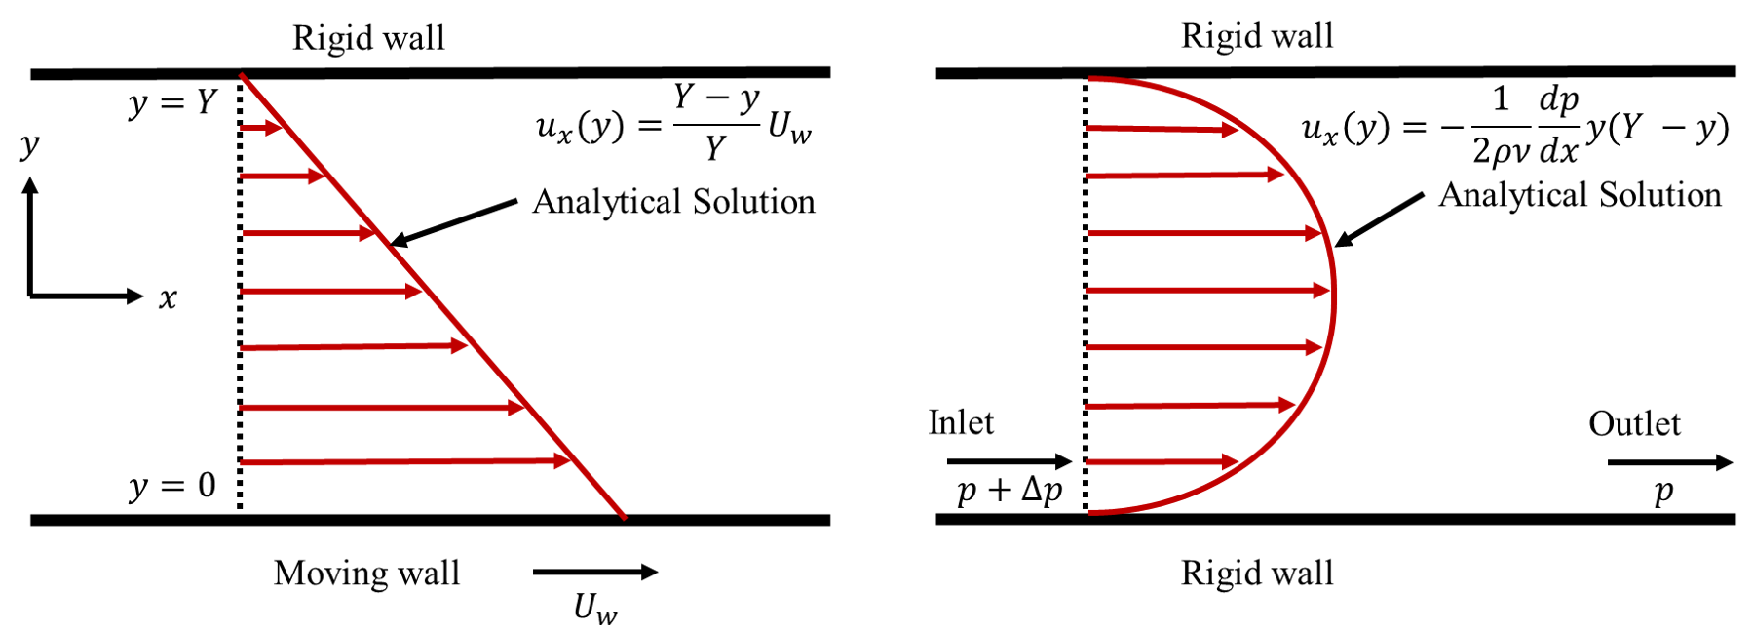
\includegraphics[width=0.98\textwidth]{imgs/couette_and_poiseuille.pdf}
  \caption{The conceptual visualizations of the Couette flow (Left) and
  Poiseuille flow (Right).}
  \label{couette-and-poiseuille-conceptual}
\end{figure}


\subsection{Couette flow}
The Couette flow is the flow between two walls as shown in
Figure~\ref{couette-and-poiseuille-conceptual}:
One is fixed and the other moves horizontally with the velocity of $U_w$.
The flow is caused by the viscous drag force acting on the fluid.
Since the Couette flow also has an analytical solution,
we can validate the implementation of the moving wall.
The analytical solution for Figure~\ref{couette-and-poiseuille-conceptual} is given by~\cite{nagy2019graphical}:
\begin{equation}
\begin{aligned}
  u_x(y) =\frac{Y - y}{Y}U_w
\end{aligned}
\end{equation}
where $Y$ is the distance between the two walls
and $u_x(y)$ is the horizontal velocity of the flow
at the location of $y$. 
In the experiment, we apply the bounce-back boundary condition
at the moving wall and the rigid wall
and the periodic boundary conditions at the inlet and outlet.
The results are shown in Figure~\ref{fig:couette-velocity-evolution}.
As shown in the figures, the flow velocity iteratively approaches
the analytical solution and it perfectly fits in the end
and the velocity stops growing as seen at $t=1600, 2000$.
From this experiment, the moving wall can be validated.

\begin{figure}[H]
  \vspace{-1mm}
  \centering
  \includegraphics[width=0.58\textwidth]{../log/couette_flow/fig/couette_flow_joint.pdf}
  \vspace{-5mm}
  \caption{The velocity evolution at
  the $x = 25$ in the lattice grid size of $(50, 50)$.
  The wall velocity $U_w$ at the bottom and the relaxation term $\omega$ are set
  to $50$ and $0.3$ respectively.
  The initial density is $\rho(\xv) = 1.0$ and the initial velocity is $\uv(\xv) = (0, 0)$. 
  \label{fig:couette-velocity-evolution}}
\end{figure}

\subsection{Poiseuille flow}
The Poiseuille flow is the flow between two non-moving walls as shown in Figure~\ref{couette-and-poiseuille-conceptual}.
The flow is caused by a constant pressure difference $\od{p}{x}$
in the horizontal direction of the two walls.
The Poiseuille flow also has the analytical solution
and we can validate the implementation of the periodic boundary conditions
with pressure variation.
The analytical solution for Figure~\ref{couette-and-poiseuille-conceptual} is given by~\cite{mendiburu2009analytical}:
\begin{equation}
\begin{aligned}
  u_x(y) = - \frac{1}{2\rho \nu} \od{p}{x} y (Y - y)
\end{aligned}
\end{equation}
In the experiment, we apply the bounce-back boundary condition
at the moving wall and the rigid wall
and the periodic boundary condition with pressure variation at the inlet and outlet.
Figure~\ref{fig:poiseuille-velocity-evolution} presents the results
and the simulated results approaches the analytical solutions as in the Couette flow.
In the end, it fits completely
and the velocity stops growing as seen at $t=4000, 5000$.

\begin{figure}[H]
  \centering
  \includegraphics[width=0.58\textwidth]{../log/poiseuille_flow/fig/poiseuille_flow_joint.pdf}
  \caption{The velocity evolution at
  the $x = 25$ in the lattice grid size of $(50, 50)$.
  The relaxation term $\omega$ are is
  to $0.7$.
  The density factor at the inlet and the density factor
  at the outlet are set to $0.3$ and $0.301$ respectively.
  The initial density is $\rho(\xv) = 1.0$ and the initial velocity is $\uv(\xv) = (0, 0)$.
  \label{fig:poiseuille-velocity-evolution}}
\end{figure}

\section{Lid-driven cavity}
Finally, we handle a concrete example.
In this paper, the lid-driven cavity shown in Figure~\ref{lid-driven-cavity-conceptual} are simulated.
The lid-driven cavity simulates the flow inside a box with
three rigid walls and one moving wall, i.e. a lid.
In this simulation, it is known that the turbulence is caused 
when the following Reynolds number is larger than 1000~\cite{chiang1998effect}:
\begin{equation}
\begin{aligned}
  \text{Re} = \frac{LU}{\nu}
\end{aligned}
\end{equation}
where $L$ is the characteristic length parameter
of the body and $U$ is the stream flow velocity.
One key property of the Reynolds number is that two flow system
is dynamically similar if the Reynolds number and the geometry are similar~\cite{kundu2008fluid}.
Therefore, we present the results with various 
viscosity $\nu$ and the wall velocity $U = U_w$ that 
satisfy the Reynolds number of $1000$ under $L = X = Y = 300$
in Figure~\ref{fig:sliding-lid-velocity-evolution}.
As the viscosity and velocity becomes larger,
the convergence becomes quicker.
On the other hand, all the settings converge to the similar flow in the end
as indicated in the key property of the Reynolds number.

\begin{figure}[t]
  \centering
  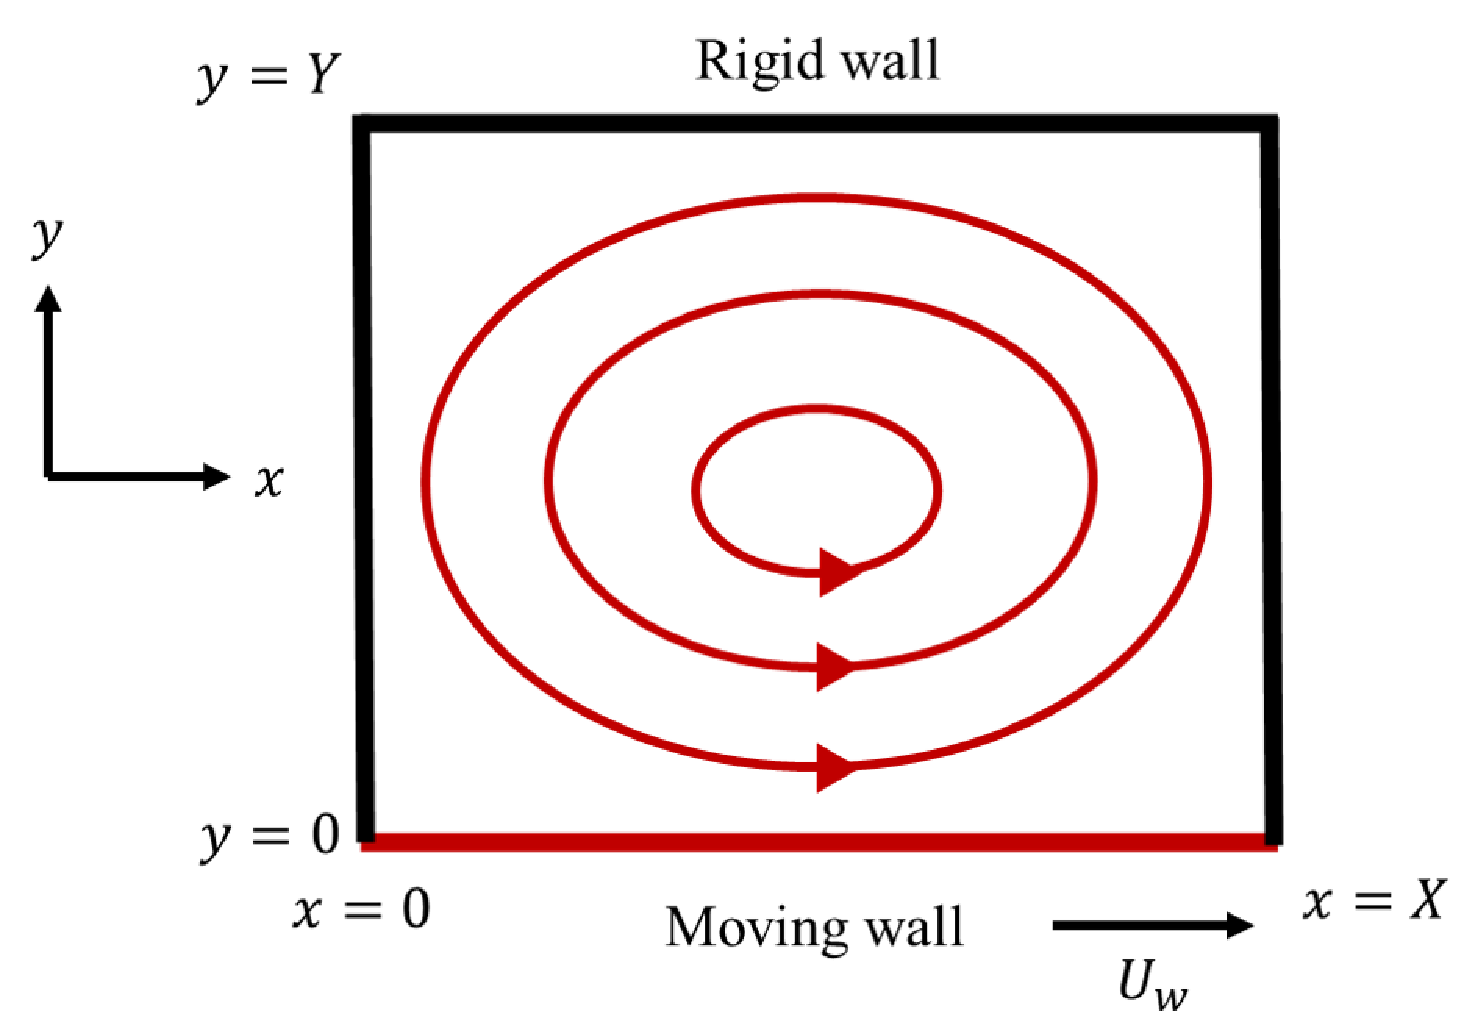
\includegraphics[width=0.48\textwidth]{imgs/lid-driven-cavity.pdf}
  \caption{The conceptual visualizations of the lid-driven cavity.}
  \label{lid-driven-cavity-conceptual}
\end{figure}

\begin{figure}[t]
  \begin{center}
    \subfloat[$U_w = 0.1, \nu = 0.03$]{
      \includegraphics[width=0.40\textwidth]{../log/sliding_lid_W0.10_visc0.03_size300/fig/vel_flow095000.pdf}
    }
    \subfloat[$U_w = 0.2, \nu = 0.06$]{
      \includegraphics[width=0.40\textwidth]{../log/sliding_lid_W0.20_visc0.06_size300/fig/vel_flow095000.pdf}
    }\\
    \vspace{-3mm}
    \subfloat[$U_w = 0.3, \nu = 0.09$]{
      \includegraphics[width=0.40\textwidth]{../log/sliding_lid_W0.30_visc0.09_size300/fig/vel_flow095000.pdf}
    }
    \subfloat[$U_w = 0.4, \nu = 0.12$]{
      \includegraphics[width=0.40\textwidth]{../log/sliding_lid_W0.40_visc0.12_size300/fig/vel_flow095000.pdf}
    }\\
    \caption{The stream plots of sliding lid
    with the lattice grid size of $(300, 300)$.
    Each setting is chosen to satisfy the Reynolds number 1000.
    The initial density is $\rho(\xv) = 1.0$ and the initial velocity is $\uv(\xv) = (0, 0)$.
      \label{fig:sliding-lid-velocity-evolution}}
  \end{center}
\end{figure}

This experiment requires long time to complete.
For example, it takes 1 hour to finish one simulation using
intel core i7--10700 and 32GB RAM.
Recall that the advantage of LBM is to allow us to compute the simulation in
parallel easily.
For this reason, we test the scalability of this simulation using
various number of processes.
Note that all the experiments related to the scaling test
are performed on {\bf BWUniCluster}
\footnote{https://wiki.bwhpc.de/e/Category:BwUniCluster\_2.0}.
The implementation follows Section~\ref{section-mpi}.
Figure~\ref{fig:sliding-lid-scaling} shows the plot of
MLUPS, a.k.a. million lattice updates per second, and
the number of processes.
Ideally, the MLUPS grows linearly with respect to the number of processes.
However, it does not happen because of the latency of the communication
and the waiting for the synchronization as described in Amdahl's law~\cite{amdahl1967validity}.
Such slow down is also seen in Figure~\ref{fig:sliding-lid-scaling}.
\begin{figure}[b]
  \centering
  \includegraphics[width=0.88\textwidth]{../log/sliding_lid_W0.10_visc0.03_size300/fig/scaling_test.pdf}
  \vspace{-3mm}
  \caption{The scaling test of the sliding lid simulation.
  The grid size is $300 \times 300$.
  The number of processes are $1 ,4 ,9 ,16 ,25 ,36 ,100 ,144 ,225 ,400$ respectively.
  Note that both axes are log-scale.
    The viscosity and the wall velocity are set to $\nu = 0.03$ and $0.1$.
    The initial density is $\rho(\xv) = 1.0$ and the initial velocity is $\uv(\xv) = (0, 0)$.
  }
  \label{fig:sliding-lid-scaling}
\end{figure}

